\section{Methods}


\begin{figure*}[!ht]
    \centering
    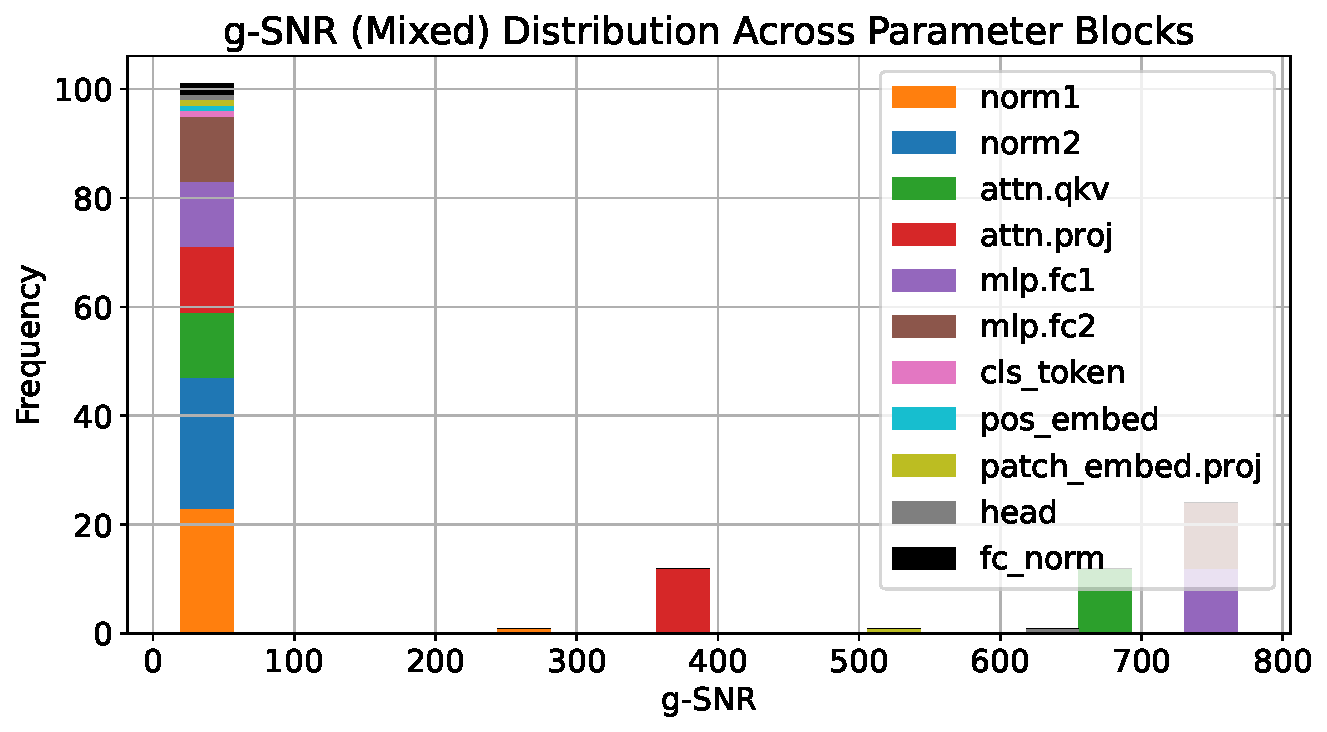
\includegraphics[width=0.33\linewidth]{images/gsnr_across_blocks_mix.pdf}
    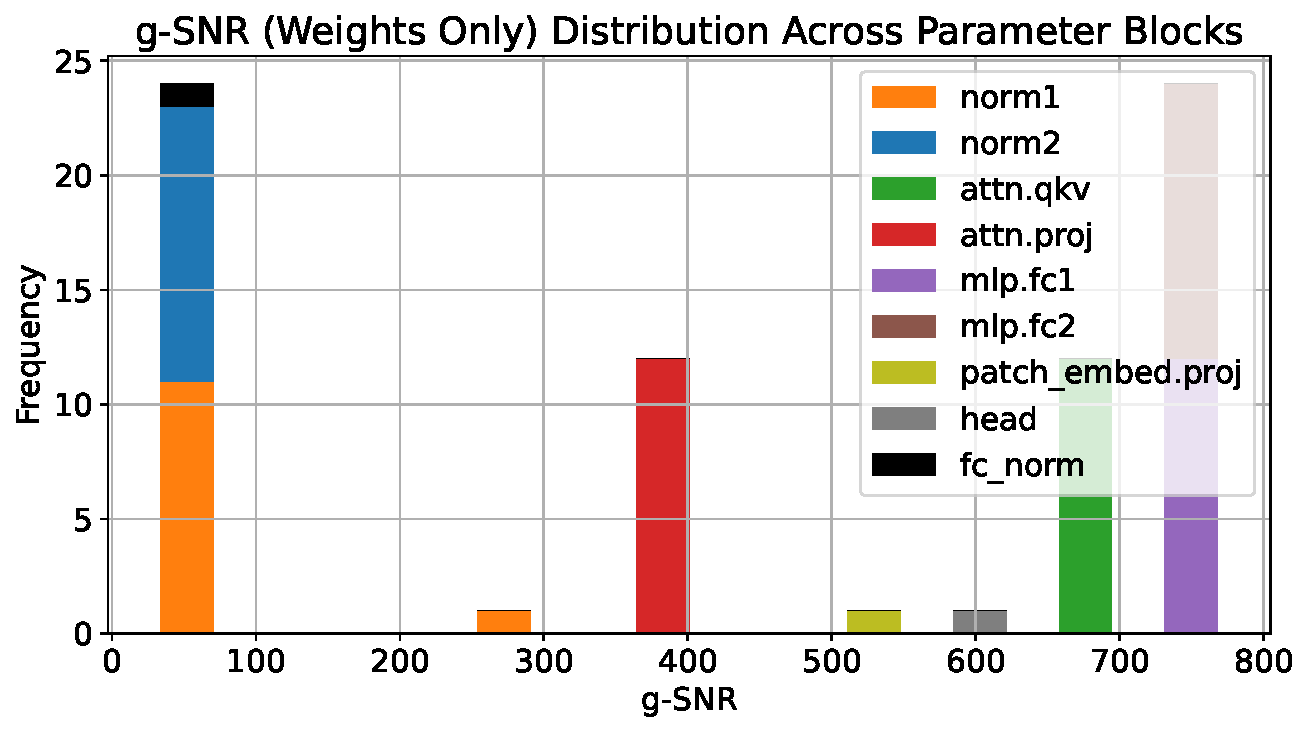
\includegraphics[width=0.33\linewidth]{images/gsnr_across_blocks_weights.pdf}
    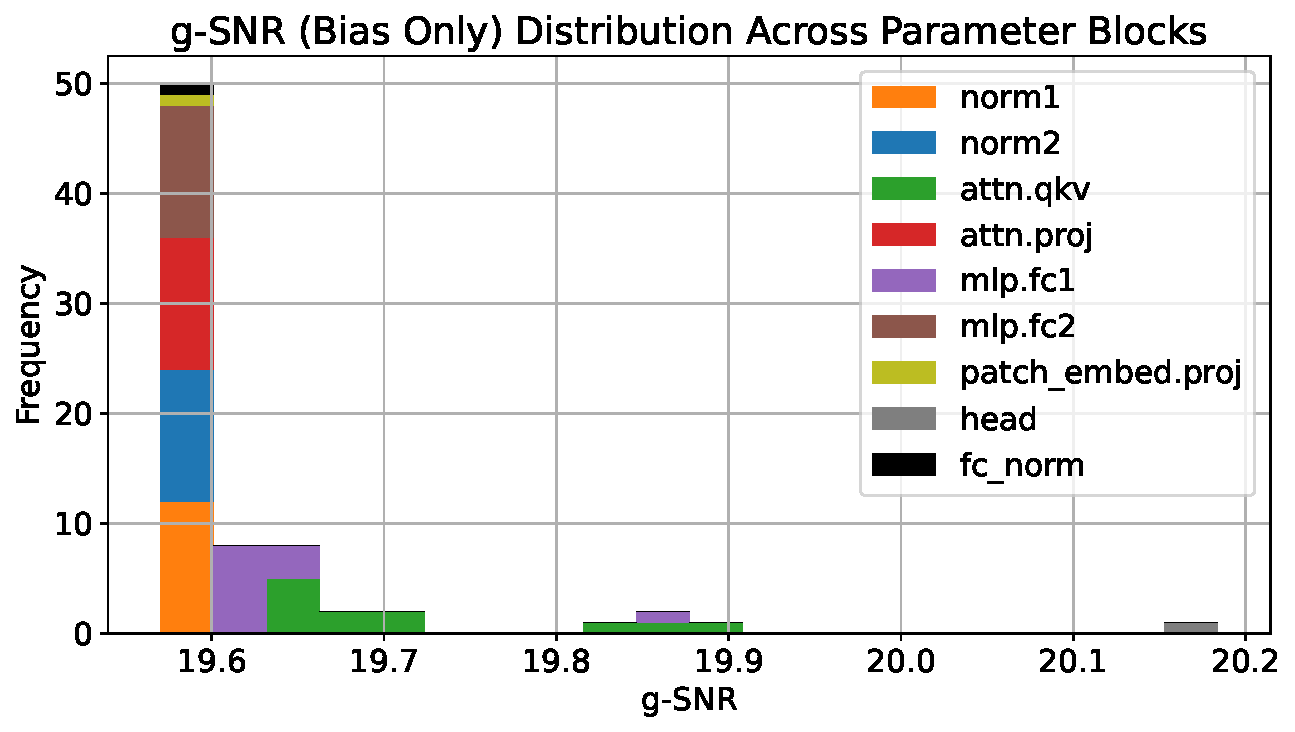
\includegraphics[width=0.33\linewidth]{images/gsnr_across_blocks_biases.pdf}
    \caption{We observe that the g-SNR varies across different parameter blocks. However, for most weights, the parameter blocks that share the same structure across different transformer layers (blocks) tend to have similar g-SNR values. Additionally, the g-SNR values for the bias parameters are consistently low magnitude. Our method can be viewed as partitioning all parameter blocks based on their structure.}
    \label{fig:gsnr_across_blocks_hist}
\end{figure*}

\begin{figure}[!h]
    \centering
    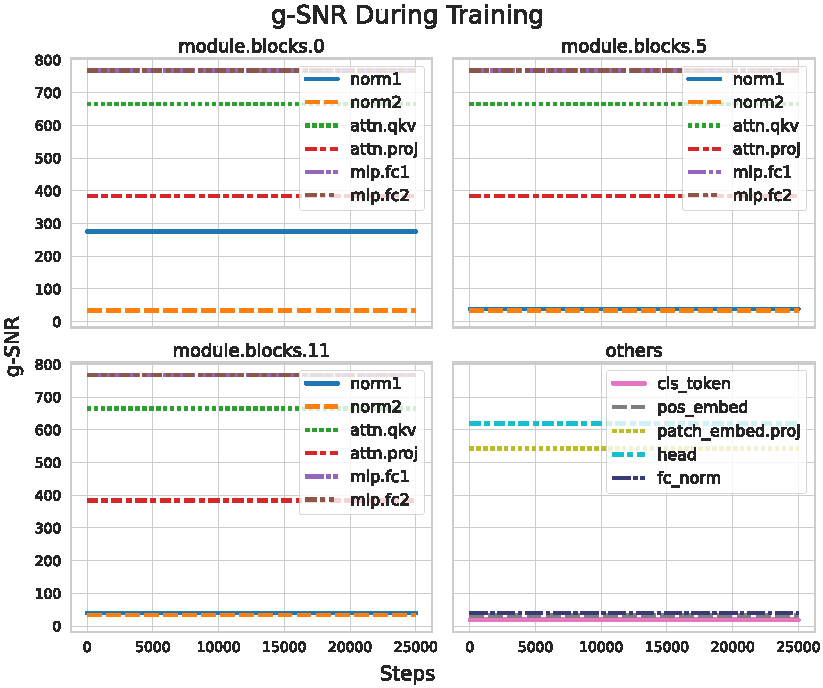
\includegraphics[width=\linewidth]{images/gsnr_analysis.pdf}
    \caption{We plot the g-SNR distribution over time for three different transformer blocks: shallow (block 0), middle (block 5), and deep (block 11). Additionally, we analyze some distinct types of parameter blocks. Our observations indicate that while the g-SNR values vary across different parameter blocks, they tend to remain relatively constant over time.}
    \label{fig:gsnr_across_time_plot}
\end{figure}


\begin{figure*}[h!]
    \centering
        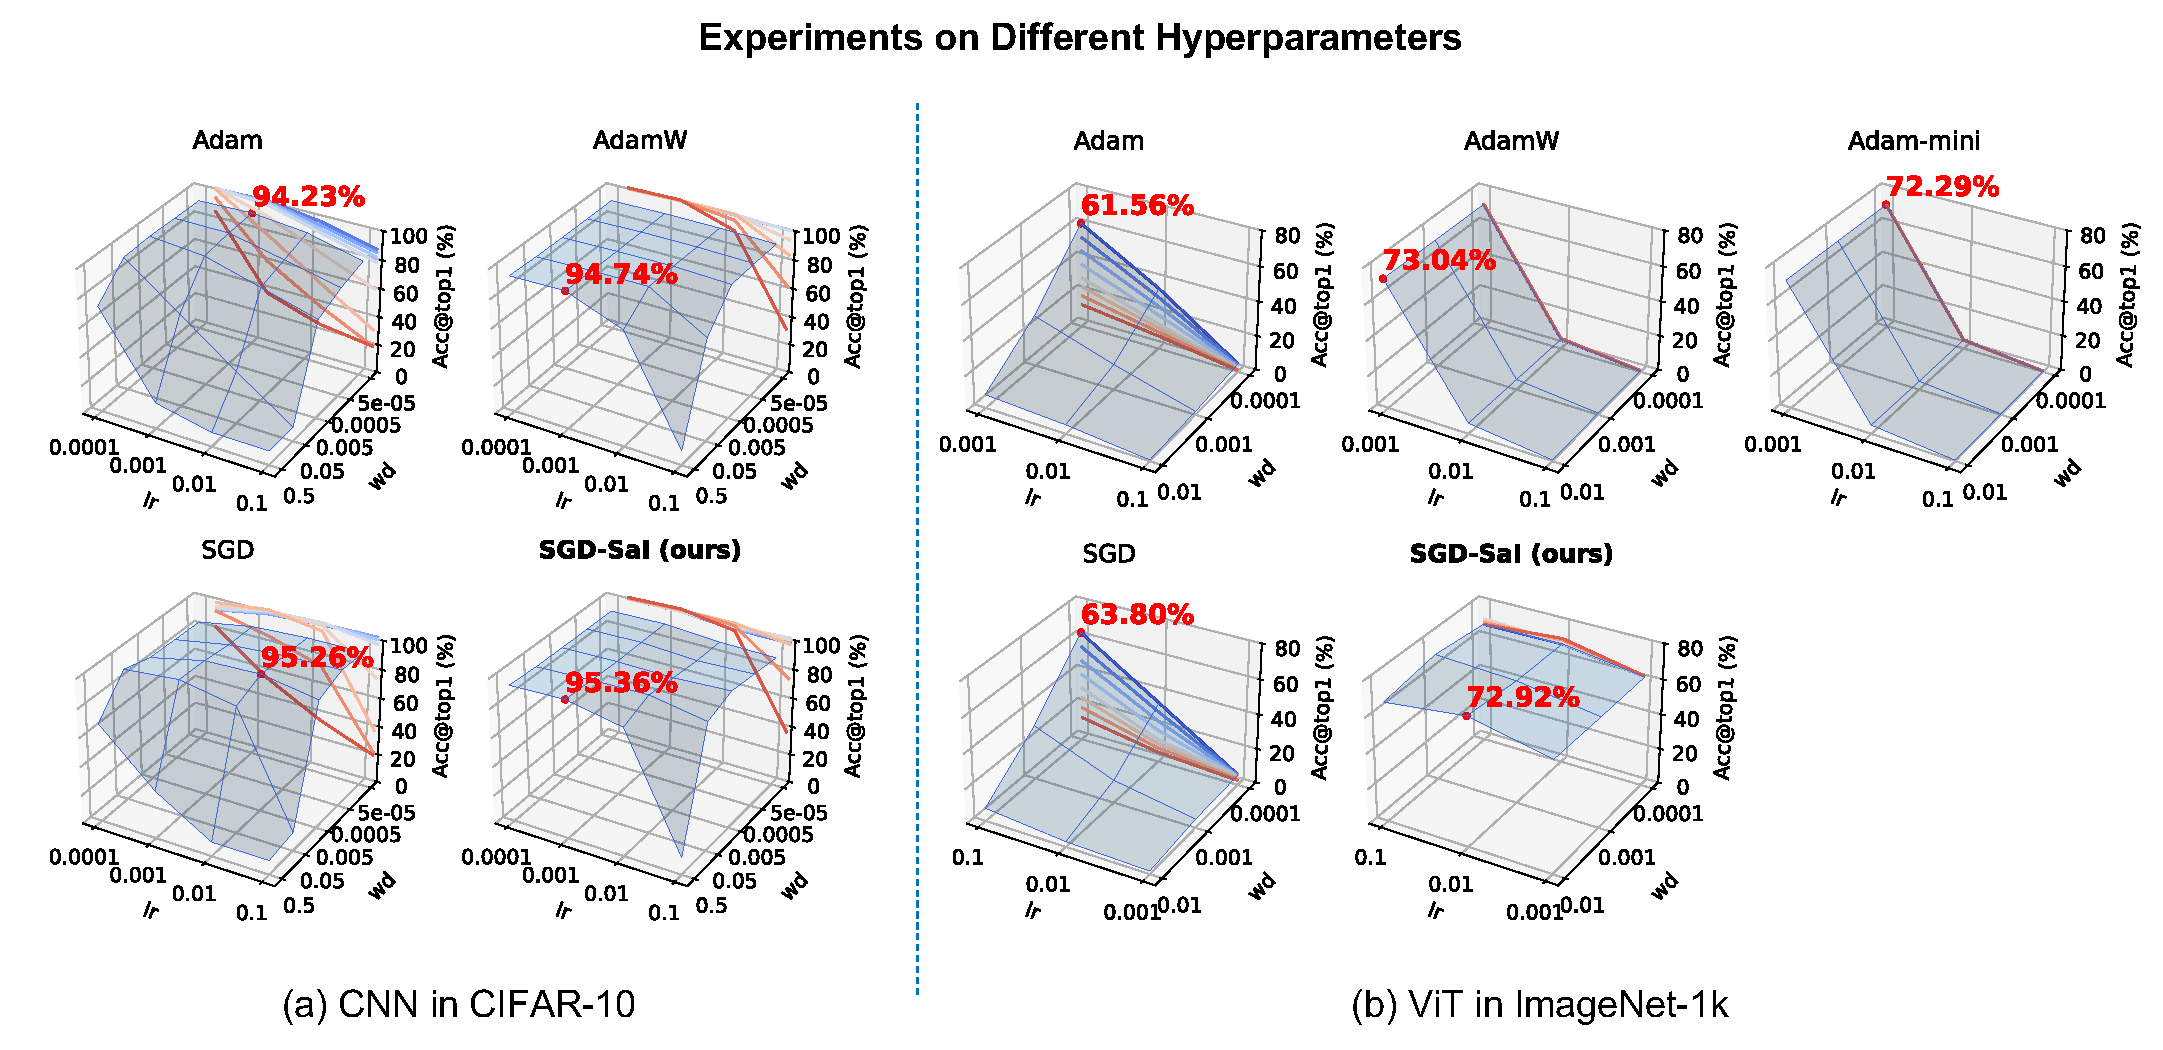
\includegraphics[width=.99\textwidth]{images/combine_3d_scatter_v3.pdf}
    \caption{Comparison of top-1 test accuracy distributions for CNNs on CIFAR-10 (Left) and ViTs on ImageNet-1k (Right) across different hyperparameter combinations. Each method demonstrates distinct performance trends, including Adam, AdamW, SGD, and SGD-SaI. Adam-Mini is only compared in the ViT case as its modification target on transformer training. SGD-SaI consistently shows enhanced robustness and performance under varying hyperparameter settings.}
    \label{fig:fig_vit_cnn_performance_3d_surface}
\end{figure*}

Considering the substantial memory overhead introduced by the second-order momentum in the Adam optimizer, this section explores strategies to reduce this cost by revisiting the foundational motivations for adaptive gradient methods.

In the following subsections, we design a memory-efficient learning rate local gain, termed g-SNR, to replace the second-order momentum. We analyse the distribution of g-SNR across different parameter groups throughout the network. This aligns with the motivation of parallel works \cite{zhang2024adamminiusefewerlearning} that focus on partitioning parameter groups for learning rate adjustment. Furthermore, we investigate the behaviour of g-SNR during training, demonstrating how dynamic local gains can be replaced with constant preconditioned values calculated in the initial iterations.

Finally, we introduce our proposed method, SGD-SaI, detailing its design and implementation. This method builds on the insights derived from g-SNR analysis, offering a memory-efficient alternative to second-order momentum while maintaining competitive performance.

\subsection{Memory Efficient Local Gain: g-SNR}
Adam builds upon RMSprop, designed to find a \textbf{local gain} for the learning rate, enabling parameter-specific adjustments within deep neural networks \cite{hinton2012neural, kingma2014adam}. By incorporating second-order momentum, Adam improves upon SGD by better handling problems with non-stationary objectives and tasks characterized by noise or sparse gradients \cite{kingma2014adam}. This mechanism allows Adam to dynamically rescale gradients, effectively adjusting the learning pace across parameter blocks with distinct gradient patterns. Consequently, Adam outperforms SGD when training architectures with heterogeneity problems in the Hessian matrix, such as Transformers \cite{zhang2024transformers, zhang2024adamminiusefewerlearning}. Another key insight arises from the warm-up mechanism: even with second-order momentum, Adam still requires a warm-up phase to reduce the learning rate at the beginning of training, aiming to mitigate gradient variance~\cite{liu2021variance}. During this phase, gradients are known to be sparse and noisy. Reducing the learning rate directly during the warm-up phase effectively lowers gradient variance, stabilizing the training process straightforwardly and efficiently.

Intuitively, adaptive gradient methods dynamically adjust the learning rate for each parameter during training. This mechanism encourages parameters with less learning history to learn more while slowing down the learning pace for parameters progressing too quickly. Essentially, it acts as a compensatory approach to address learning imbalances across parameters after they arise. However, if we can predict and pre-empt these imbalances before they occur, we could potentially eliminate the need for second-order momentum, which relies on learning history to evaluate and correct them. 

Considering the root cause of why learning imbalance occurred across different parameters, we discussed them in two main parts. Firstly, as inherited from the architecture characteristics, the parameter in different layers or with different architectures will receive distinct gradient pattern~\cite{tanaka2020pruning, lizico, xiang2023exploiting}, thus bringing the optimal learning rate for different parameters are distinct and need to be re-adjust with local gain~\cite{hinton2012neural}, Secondly, within the parameter groups, the gradient can be noisy or sparse based on the objective and data, that will introduce imbalance update to parameters.

We propose using the gradient signal-to-noise ratio (g-SNR) introduced by \cite{xiang2023exploiting} to adjust the learning rate block-wisely, as it measures the norm and variance of gradients of the parameter block, which reflects overall update magnitude and variance of gradient between paramters. Specifically for each block~$i$, the gradient norm ($\ell^2$-norm) and variance are calculated as
\[
G_{\text{norm}}^{(i)} = \sqrt{\sum_{j=1}^{d_i} \left( g^{(i)}_j \right)^2}, \quad G_{\text{var}}^{(i)} = \frac{1}{d_i} \sum_{j=1}^{d_i} \left( g^{(i)}_j - \bar{g}^{(i)} \right)^2,
\]
where $\bar{g}^{(i)} = \frac{1}{d_i} \sum_{j=1}^{d_i} g^{(i)}_j$, and $d_i$ is the number of parameters in block~$i$. The gradient signal-to-noise ratio for each block is then given by
\[
G_{\text{snr}}^{(i)} = \frac{G_{\text{norm}}^{(i)}}{\sqrt{G_{\text{var}}^{(i)}} + \epsilon},
\]
where $\epsilon$ is a small constant added for numerical stability. To ensure consistent scaling across all blocks, we normalize the g-SNR of each block by the maximum g-SNR among all blocks:
\[
\tilde{G}_{\text{snr}}^{(i)} = \frac{G_{\text{snr}}^{(i)}}{\max_{k} G_{\text{snr}}^{(k)}}.
\]
This normalization confines the g-SNR values between 0 and 1, facilitating a fair comparison and adjustment of learning rates across different parameter blocks. Thus, we establish the local gain by replacing $v_t$ with the following expression:
\begin{align*}
    \alpha^{(i)}_t = \mathcal{F}(g^{(i)}_t) = \tilde{G}_{\text{snr}}^{(i)}
\end{align*}
where $\alpha^{(i)}_t$ represents the local gain at step $t$ guided by the temporal value $\tilde{G}_{\text{snr}}^{(i)}$  which determines the update direction $\mathbb{D}_t$. This approach reduces the memory overhead of $v_t$ from $\mathcal{O}(d)$ to $\mathcal{O}(B)$. 

Adapting the learning rate according to the normalized gradient signal-to-noise ratio significantly influences gradient variance during training. When the high gradient noise or sparsity in block~$i$ occurs, $\tilde{G}_{\text{snr}}^{(i)}$ tend to have relatively lower value, the learning rate $\eta$ is scaled down by a factor $\alpha^{(i)} = \tilde{G}_{\text{snr}}^{(i)}$, resulting in a reduced learning rate $\eta^{(i)} = \alpha^{(i)} \eta$. This adjustment decreases the magnitude of parameter updates for that block:
\[
\theta^{(i)}_{t+1} = \theta^{(i)}_t - \eta^{(i)} \nabla_{\theta^{(i)}} L(\theta_t).
\]
Lowering the learning rate mitigates the amplification of gradient noise, thereby reducing gradient variance within each training step, leading to smoother convergence and enhanced robustness \cite{liu2019variance}. If $\tilde{G}_{\text{snr}}^{(i)}$ remains low across multiple batches, the continued reduction of $\eta^{(i)}$ further stabilizes training by preventing large, erratic updates.

\subsection{Statistics Analysis for g-SNR}
Building on the insights above, we implemented the g-SNR mechanism using PyTorch's Default Partition \cite{zhang2024adamminiusefewerlearning}, which computes g-SNR within each parameter block and dynamically re-scales the learning rate accordingly. To assess its effectiveness, we conducted experiments on Vision Transformer (ViT) pre-training tasks using ImageNet-1K, selecting ViT/S-16 for comprehensive tracing and analysis of gradient patterns throughout the training process.

Our analysis revealed that g-SNR remains relatively stable over time while exhibiting distinct patterns across different parameter classes, as shown in Fig.~\ref{fig:gsnr_across_time_plot}. Specifically, we examined transformer blocks from shallow, middle, and deep layers within the network and parameters outside the transformer blocks, such as positional embeddings. 

Given the g-SNR definition we provide in the previous subsection, we analyze its behaviour as follows: As modern initialization schemes (e.g., Xavier~\cite{kumar2017weight}, Kaiming~\cite{he2015delving}) ensure that at \( t=0 \):
\[
G_{\text{norm}}^{(i)}(0) \quad \text{and} \quad G_{\text{var}}^{(i)}(0)
\]
are well-controlled. This implies that \(G_{\text{snr}}^{(i)}(0)\) starts from a stable, architecture-driven ratio. During the training process, parameters are updated and controlled by the step size \(\eta\) is the learning rate. Assuming \(\eta\) is sufficiently small to stabilize training process, we have \( \theta^{(i)}_{t+1} \approx \theta^{(i)}_{t} \). Thus, the change in parameters per iteration is small.Consider the gradient at iteration \( t+1 \):
\[
\mathbf{g}^{(i)}_{t+1} = \nabla_{\theta^{(i)}}L(\theta_{t+1}).
\]
Consider a first-order Taylor expansion of the gradient around \(\theta^{(i)}(t)\):
\[
\mathbf{g}^{(i)}_{t+1} \approx \mathbf{g}^{(i)}_{t} + J^{(i)}_{t}\Delta \theta^{(i)}_{t},
\]
where \(J^{(i)}_{t}\) is the Jacobian 
(or a first-order sensitivity matrix) of \(\mathbf{g}^{(i)}\) w.r.t. \(\theta^{(i)}\), and \(\Delta \theta^{(i)}_{t}=\theta^{(i)}_{t+1}-\theta^{(i)}_{t}\). Since \(\|\Delta \theta^{(i)}_{t}\|\) is small, the change in the gradient vector is also small. Hence,
\[
g_{j(t+1)}^{(i)} \approx g_{j(t)}^{(i)}, \quad \forall j.
\]
Because each component \( g_{j(t+1)}^{(i)} \) differs only slightly from \( g_{j(t)}^{(i)} \), their average and variance remain stable:
\[
\bar{g}^{(i)}_{t+1} \approx \bar{g}^{(i)}_{t}, \quad
G_{\text{var}(t+1)}^{(i)} \approx G_{\text{var}(t)}^{(i)}.
\]

Similarly, for gradient norm,
\[
G_{\text{norm}(t+1)}^{(i)} = \sqrt{\sum_{j=1}^{d_i} \bigl(g_{j(t+1)}^{(i)}\bigr)^2} \approx G_{\text{norm}(t)}^{(i)}.
\]

Since both \( G_{\text{norm}(t)}^{(i)} \) and \( G_{\text{var}(t)}^{(i)} \) remain nearly unchanged,
\[
G_{\text{snr}(t+1)}^{(i)} = \frac{G_{\text{norm}(t+1)}^{(i)}}{\sqrt{G_{\text{var}(t+1)}^{(i)}}+\epsilon} \approx \frac{G_{\text{norm}(t)}^{(i)}}{\sqrt{G_{\text{var}(t)}^{(i)}}+\epsilon} = G_{\text{snr}(t)}^{(i)}.
\]

Thus, \(G_{\text{snr}(t)}^{}\) remains effectively constant over iterations. Even though parameters change, the "shape" or statistical profile of the gradient distribution does not drastically alter. The g-SNR measures a dimensionless ratio that characterizes this shape. Minor parameter shifts do not significantly affect this ratio; hence, it remains nearly constant.


This finding aligns with the observation by \cite{xiang2023exploiting} that g-SNR strongly correlates with architecture. Leveraging this insight, we replaced the dynamic calculation of g-SNR with constant values determined during initialization, significantly reducing computational costs during each training step.

When calculating g-SNR using PyTorch's Default Partition, we observed that the g-SNR values vary significantly across partitions. By leveraging constant g-SNR values, this approach effectively assigns a pre-conditioned learning rate scale to each partition. \cite{zhang2024adamminiusefewerlearning} highlights a key limitation of PyTorch's default parameter partitioning: its lack of granularity for optimizers like Adam-mini. While PyTorch groups parameters such as attention QKV together, Adam-mini requires finer partitions, such as by attention heads or neurons, to perform effectively, especially in Transformer-based architectures. This limitation stems from the default partitioning's failure to align with Hessian sub-block structures critical for optimization.

This observation does not hold true in our case. Our empirical results, shown in Fig.~\ref{fig:fig_vit_cnn_performance_3d_surface} and discussed further in Sec.~\ref{sec:results}, demonstrate that our method works effectively with PyTorch's Default Partition and does not require any additional fine-grained partitioning strategies. The distribution of g-SNR across different partitions is detailed in Fig.~\ref{fig:gsnr_across_blocks_hist}, where we observe that, for most weights, parameter blocks sharing the same structure across different Transformer layers exhibit similar g-SNR values. Additionally, the g-SNR values for bias parameters remain consistently low, reflecting their uniform magnitude. A notable exception is the $norm1$ weights from $blocks.0$, which connect to the input from embedded patches, whereas all other $norm1$ weights connect to the output of the previous block. This observation highlights that our g-SNR values can effectively identify distinct characteristics among different parameter groups and the network's topological impacts. Moreover, it indicates that gradient sparsity and noise levels vary across parameter groups, confirming the necessity of using a local gain mechanism to balance learning rates across partitions.

Notably, our approach, compatible with PyTorch's Default Partition, enables simultaneous updates of each coarse-grained parameter block and eliminates the need for dynamic learning rate calculations. This efficiency resulted in a threefold speedup in the optimizer update step compared to Adam-mini when training the GPT2-small model. Moreover, it reduces the implementation complexity associated with the exhaustive Hessian calculations required for fine-grained parameter partitioning \cite{zhang2024adamminiusefewerlearning}.

In summary, instead of relying on second-order momentum to compute gradient history and adjust learning rates to address imbalanced updates after they occur, our g-SNR approach determines the gradient sparsity level at the first iteration of training. This enables assigning appropriate pre-conditioned learning rate scales to different parameter partitions, simplifying the update process, improving memory efficiency, and significantly speeding up optimization.



\subsection{Proposed Methods Detail: SGD-SaI}
We propose a new method called \textbf{SGD-SaI} that removes adaptive gradient components by rescaling the learning rates of each parameter block using the g-SNR calculated from the initial batch. The algorithm details are presented in Algorithm~\ref{algo:algorithm_cmp}. By leveraging the initial g-SNR, we capture the inherent gradient characteristics of different parameter blocks, allowing for a constant scaling factor that addresses the variations in gradient magnitudes across blocks.

As our method eliminates the dynamic terms associated with adaptive gradient algorithms, it only introduces a few computations at the first iteration compared to naive Stochastic Gradient Descent with Momentum (SGDM). Specifically, the additional computation involves calculating the g-SNR for each parameter block during the initial batch. After this initial computation, the training proceeds similarly to standard SGDM, making our method computationally efficient and comparable in complexity to traditional SGD.

To update the g-SNR based on the actual gradient sparsity without affecting the gradient computation, we adopt \textbf{decoupled weight decay} as proposed by Loshchilov and Hutter~\cite{loshchilov2019decoupled}. Decoupled weight decay applies regularization directly to the parameters rather than incorporating it into the gradient computation. This approach is equivalent to regularization in SGD and allows us to accurately compute the gradient statistics needed for the g-SNR without the weight decay term distorting the gradient values. By doing so, we ensure that the g-SNR reflects the gradients' true sparsity and noise characteristics.

Our implementation remains extremely straightforward, as we adopt the simplest approach that requires only minimal modifications to the existing SGD optimizer. This simplicity ensures that existing tricks and frameworks that support SGD can seamlessly integrate with and support our method.
\begin{figure}[!ht]
    \centering
    % % Proposed algorithm
    \begin{minipage}{0.45\textwidth}
        \begin{algorithm}[H]
            \caption{SGD-SaI}\label{algorithm:sgd_boost}
            \footnotesize
            \begin{algorithmic}[1]
                \Require $T$ (total steps), $\eta$ (learning rate), $\theta^i$ ($i$-th parameter block), $L(\theta)$ (loss function), $\lambda$ (weight decay), $\mu$ (momentum), $\epsilon$ (small constant), $maximize$
                \For{$t \gets 1$ to $T$}
                    \State Compute gradient: $g^i_t \gets \nabla_{\theta^i} L(\theta_{t-1})$
                    \If{$maximize$}
                        \State $g^i_t \gets -g^i_t$
                    \EndIf
                    \State \text{/* Apply momentum */}
                    \If{$t > 1$}
                        \State $m^i_t \gets \mu m^i_{t-1} + (1 - \mu) g^i_t$
                    \Else
                        \State $m^i_t \gets g^i_t$
                        \State \text{/* Compute g-SNR */}
                        \State $G_{\text{snr}}^i \gets \dfrac{G_{\text{norm}}^i}{\sqrt{G_{\text{var}}^i} + \epsilon}$
                        \State \text{/* Normalize g-SNR */}
                        \State $\tilde{G}_{\text{snr}}^i \gets \dfrac{G_{\text{snr}}^i}{\max_k G_{\text{snr}}^k}$
                    \EndIf

                    \State \text{/* Apply weight decay */}
                    \State $\theta^i_t \gets \theta^i_{t-1} - \lambda \eta \theta^i_{t-1}$
                    \State \text{/* Update parameters with scaled learning rate */}
                    \State $\theta^i_t \gets \theta^i_t - \eta \tilde{G}_{\text{snr}}^i m^i_t$
                \EndFor
            \end{algorithmic}
        \end{algorithm}
    \end{minipage}
    \caption{Our Algorithm. we introduce a simple parameter-block-wise scaling using the normalized g-SNR to rescale the learning step size. This allows SGD to perform block-wise effective learning, unlocking its potential to work well on networks with block heterogeneity problems~\cite{zhang2024transformers}.}
    \label{algo:algorithm_cmp}
\end{figure}

